\documentclass[11pt]{article}

\usepackage{fullpage}
\usepackage{enumitem}
\usepackage{graphicx,wrapfig}

\begin{document}

\title{ARM Final Report}
\author{
  Abhinav Mishra,
  Arthur-Mihai Niculae,
  Szilveszter Szekely,
  Tom Bellingham
}

\maketitle

\section{Introduction}

\section{Assembler}

\subsection{Design}

The assembler has been implemented according to the two pass design provided in
the specification file. However we read the input file only once and iterate
over the stored instructions twice.

The assembler has four major components:
\begin{itemize}[noitemsep,topsep=0pt]
  \item \textbf{Tokenizer}:
    to tokenize the instruction.
  \item \textbf{Parser}:
    to parse the tokenized instruction.
  \item \textbf{Dictionary}:
    to look for the mnemonics and their respective values.
  \item \textbf{Instruction Generator}:
    to generate the final binary encoding.
\end{itemize}

\subsection{Implementation}

Every line in the instruction is fed into the tokenizer which returns a list
of tokens. These tokens are then passed to the parser which recognizes the
mnemonic and parses the whole instruction into a usable format. While the
instruction is being parsed the dictionary is used extensively to classify the
tokens. Once the instruction has been parsed, it is passed to the instruction
generator which connects all the components of the parsed tokens and generates
a final binary encoding of the instruction.

In this implementation of the assembler, majority of the data structures are
being reused from the emulator.

\subsection{Extensions}

The assembler has been extended to implement some more instructions comments.
All the instructions are now of the type:
\textbf{opcode\{cond\} \{operands\}}
\begin{itemize}[noitemsep,topsep=0pt]
  \item \textbf{opcode}: Basic Instruction
  \item \textbf{cond}: Ex: eq, hi, al, cc, etc.
  \item \textbf{operands}: Ex: registers, immediate values.
\end{itemize}
Example: andeq r0, r0, r0, mulhi r1, r2, r3.

It also supports comments along with the instructions which can be used to
explain the code.

\section{Extension}

\subsection{Acknowledgement}

We gratefully acknowledge those  whose libraries and tutorials have been used
to help make this extension.

\begin{itemize}[noitemsep,topsep=0pt]
  \item \textbf{Cambridge University Tutorials} for Baking Pi –
    Operating Systems Development.
  \item \textbf{Valvers.com} for Bare Metal Programming in C.
  \item \textbf{Brian Sidebotham} for Raspberry Pi Baremetal Libraries.
  \item \textbf{Linux Devs} for checkpatch.pl utility
  \item \textbf{PiFox Team} for imager.py utility
  \item \textbf{D. Richard Hipp} for makeheaders utilility
\end{itemize}

\subsection{Description}

Our extension features graphical output driven by our own software renderer, in
combination with controller input, to provide a competitive multiplayer bare
metal mini-game experience.

It is a simple multiplayer survival arcade game where you have to avoid the
obstacles and stay alive for as long as possible.

\subsection{Design Decisions}

\begin{wrapfigure}{r}{5cm}
  \caption{Current Gameplay}\label{wrap-fig:1}
  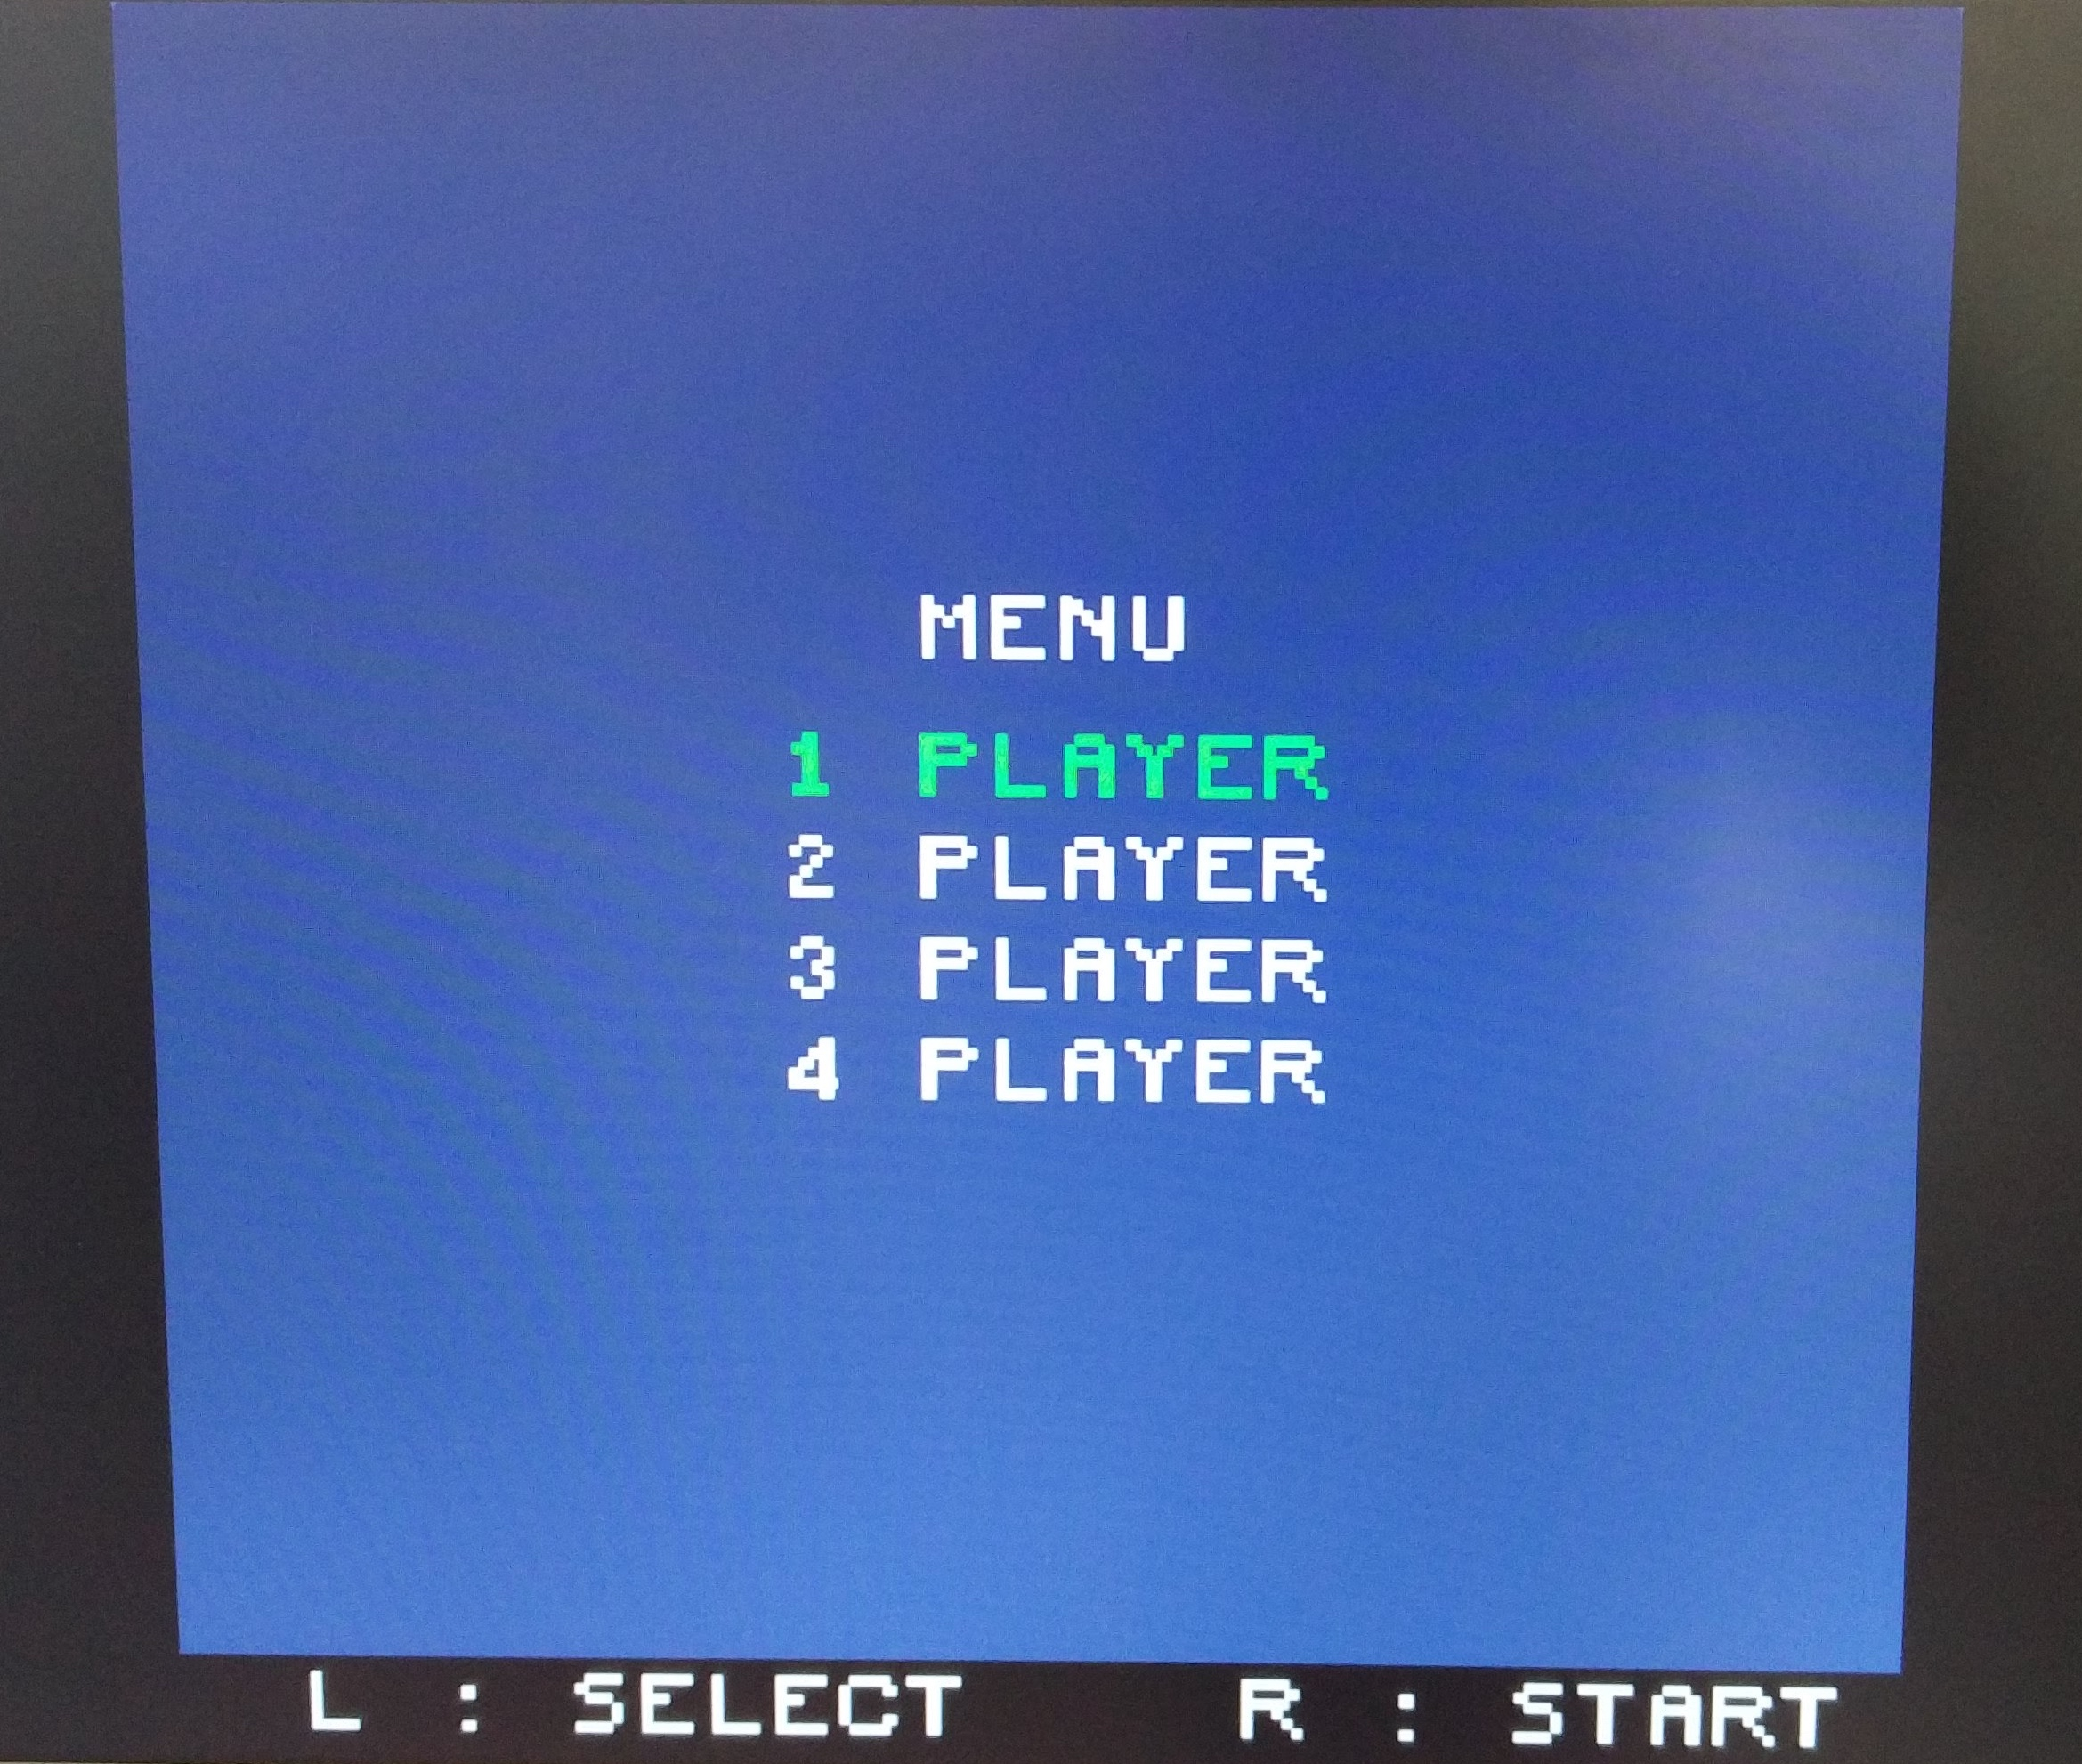
\includegraphics[width=5cm]{menu}
  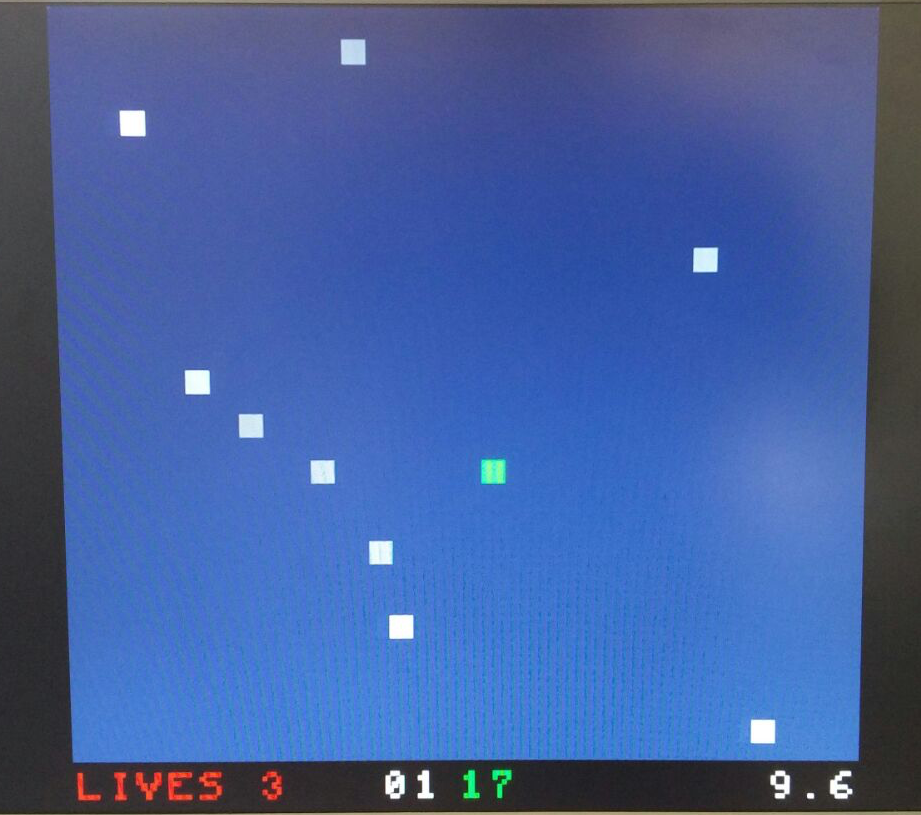
\includegraphics[width=5cm]{screen}
\end{wrapfigure}

Our objective has been to learn about and exploit as many facets of the
Raspberry Pi's functionality as possible; pursuing an interactive experience
enabled us to do this effectively by compartmentalising research and
implementation tasks between group members. We initially hoped to make use of
graphics, sound, and controller input.

Due to time constraints and implementation challenges, we continually altered
and evolved our ideas to accommodate a range of Pi functionality whilst still
building an interactive experience.

\subsection{Testing Methodology}

Testing our program has been a challenging experience. The main method has been
compiling our program, putting it on the Pi and running it. This has proven
adequate in most cases, where we only had to debug our application logic, so we
could see what appears on the screen. However in some specific cases it did turn
out be not enough.

For some parts the strategy has been to compile it for \texttt{x86\_64}. This
consisted of stubbing out the parts that natively interface with the board and
then compiling the code for our machines while changing compiler flags. Now
using a native executable we could step through the code with \texttt{gdb}.

But this was no help when trying to test the board's peripheral functionalities.
We tested that using trial and error only with some very simple output, for
example painting the screen a given color and then spinning to prevent further
statements from being executed.

After implementing our own print function, testing became easier for us.
We used it to output certain variables and string onto the screen and check
their values. This method helped us rectify the GPIO Input, the frame rate and the
timer in our project.

\subsection{Implementation Challenges}

Initially we had a lot plans on what we want to do. As the project progressed on
these came more and more in line on what we could do realistically. We had to
scrap some features while also gaining some new ones instead that we could
implement.

Lack of documentation regarding specific parts had a negative effect.  For
example our first idea was to use multi axis joysticks for input but we had to
abandon the idea because there was no documentation available on how the pins
are supposed to be used.

Implementing some features such as DMA and GPIO has been challenging because of
the previously mentioned testing deficiencies. When developing for our machines
we had access to tools such as \texttt{gdb} and \texttt{valgrind} that greatly
facilitate finding errors in our code. As these were not available on bare metal
we had to resort to trial and error debugging.

However in cases where it was possible compiling for our machines has been
a great help. We had a bug in our software rasterizer (still outstanding at the
time this report is written), where the colors in the triangle are not
interpolated correctly. We have verified that on our machines the colors render
properly and therefore that we should focus on what is done differently on Pi.

\section{Group Reflection}

\subsection{Communication}

We established clear communication channels, but early on only sporadically
shared progress updates, reading material, design suggestions, and other ideas.
Over time we synchronised our enthusiasm and focus, thus meeting in person
often and for long periods of time. Group members were occasionally late to
arranged meetings or didn't respond to messages, which caused minor delays, but
in the final weeks we cooperated seamlessly with constant feedback, discussion,
and meetings.

\subsection{Participation}

Tasks I and II were handled disproportionately between members, partly due to
discrepancy in programming ability, and partly due to unfortunate time
commitments external to the project. However, partitioning the extension into
workable chunks was then streamlined - some tasks we tackled together and
others were delegated to individual members depending on ability and
confidence. The freedom to shape the project as we imagined allowed us to
distribute tasks more effectively.

\subsection{Reflection}

This project has exposed many challenges of coordinating within a team of
varied abilities. We now aprehend how important it is to understand the talents
of each group member before allocating tasks, and how crucial it is to actively
support each other. We learned to empathsize with each other when frustrations
arose, and to persevere despite waning enthusiasm. Our initial communication
patterns were irregular, and we have learned that solid conversation binds
a team together. In future, we would like to maintain the habit of giving each
other constant feedback, collaboratively making high-level decisions, and
cooperating merrily despite differences in ability, language, or personality.

\section{Personal Reflection}

\subsection{Abhinav Mishra}

Coming from 4 months of Java, learning and getting used to C was not very easy
for me. But due to the unavailability of some of our team members I didn't have
the time to learn C first and then work on the project.

This group project has been challenging us since day one. We tried to complete
assembler and emulator in parallel to quickly move to the extension, So I had
to handle the assembler single handedly and I am proud of the fact that I was
able to complete integral parts of the project and implement some nice designs.

Overall I would say that this has been a really challenging and rewarding
project. We as a team managed to overcome each other's weaknesses and complete
the project.I got to learn a lot about Raspberry Pi's, GPIO, Graphics and C.
Thinking about the future projects I would like to be more communicative and
discussive of my ideas and try to get work done on time.

\subsection{Arthur-Mihai Niculae}

I didn’t have problems teaching myself a new language, but I was discouraged
when teammates finished tasks that were assigned to me. In future, I need to
ask about some details of implementation and not make assumptions (e.g.
I worked for a day writing a sound player in C, but didn’t realize that we did
not have access to system calls in our bare metal implementation). Following
the WEBPA assessments I learned that when I am not sure what to focus on,
I should strive to help my teammates with tasks that they are undertaking or
research better approaches in order to improve code quality. I learned a lot
about topics in which I didn’t have any previous experience (e.g. DMA,
framebuffer, multithreading and parallel processes), but sometimes I didn’t
have time or they were too complicated to implement in a short span of time.

\subsection{Szilveszter Szekely}

I was one of the most experienced members of the group, but this also became
a disadvantage in the beginning. As I rushed ahead with the implementation of
the tasks I did not communicate enough with my teammates which created friction
in our group. This has been reflected in my WebPA feedback. After we discussed
this issue I tried taking an approach that more heavily relies on group work
rather than me doing things on my own. By the time this report is written
I believe I have gotten to a point where I can more fluidly work with my
teammates.

My experience also yielded, in my opinion, significant benefits. I argued
strongly for some design decisions that were initially inconvenient, but had
long term positive consequences. For example, arguing for using checkpatch from
Linux generated lots of style errors that had to be fixed in the beginning, but
our codebase now has a consistent style.

\subsection{Tom Bellingham}

\end{document}
